\chapter{Nonlinear Dimensionality Expansion}
% Authors: Hongyu (Florence) Lu, Michael Gold, Erica Dominic.
% Lecture date: 1.28.19

\section{Motivation}
% Authors: Hongyu (Florence) Lu, Michael Gold, Erica Dominic.
% Lecture date: 1.28.19

A network is ``deep'' if it has more than one stage of non-linear feature transformation. A natural question arises: why are deep networks necessary?
Theoretically, kernel machines can approximate any function with as much precision as desired.
However, that might be computationally expensive---too expensive to achieve anything in practice.

\subsection{Cover's Theorem}
% Authors: Hongyu (Florence) Lu, Michael Gold, Erica Dominic.
% Lecture date: 1.28.19

One way to rectify this problem is to bring the sample data into a higher dimension.
Thomas Cover's theorem (1965) formalized this argument.

\textbf{Cover's Theorem:} say you have a linear classifier in $N$ dimensional space with $P$ sample points, each randomly labeled with one of two class labels.
Then \cref{fig:covers_theorem} roughly illustrates the probability that these points are linearly separable.

\begin{figure}[ht]
\centering
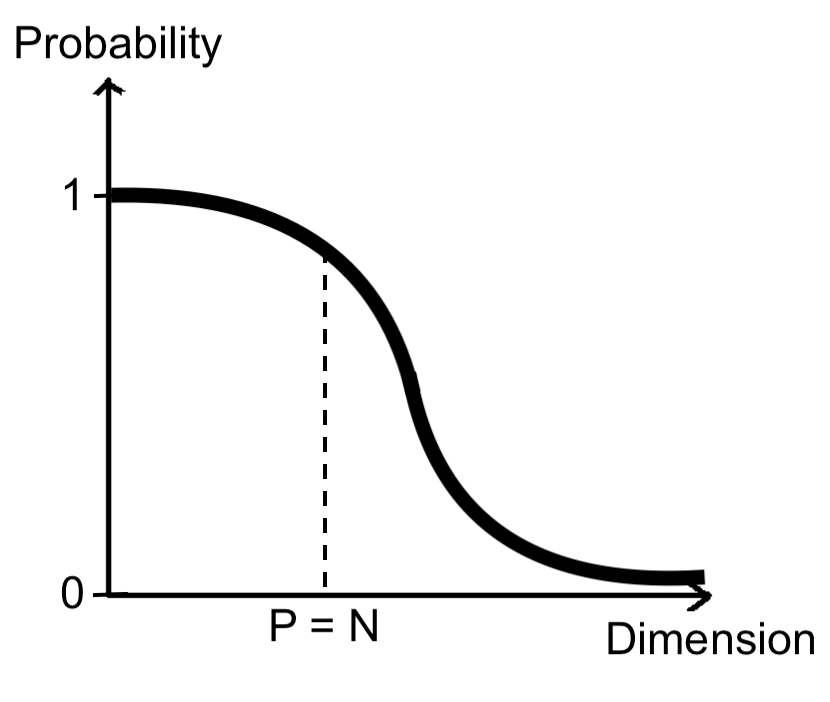
\includegraphics[width=40mm]{lectures/01-b/covers_theorem.png}
\caption{Cover's Theorem: probability of being separable vs. dimension}
\label{fig:covers_theorem}
\end{figure}

Ergo it makes sense to expand dimensionality of a representation because the data is more likely to be separable in a higher dimensional space.
One caveat: the expansion must be \emph{nonlinear}.
That brings us to deep networks, which by definition are networks with more than one nonlinear stage.

\subsection{The Manifold Hypothesis}
% Authors: Hongyu (Florence) Lu, Michael Gold, Erica Dominic.
% Lecture date: 1.28.19

Before we discuss how to expand dimensionality in a nonlinear way, we should address one concern: will working in a higher introduce an intractability problem?
The manifold hypothesis suggests that it will not pose a problem.
The manifold hypothesis postulates that natural data in high-dimensional space generally has a low-dimensional structure (see \cref{chp: manifold_hypothesis} for further discussion).
The shape of that low-dimensional space is dictated by the intrinsic factors of variation in the data, and our ideal feature extractor would extract those factors of variation.

\section{How to Expand Dimensionality Nonlinearly}\label{sec: expand_dim}
% Authors: Hongyu (Florence) Lu, Michael Gold, Erica Dominic.
% Lecture date: 1.28.19

As described in the previous section, Cover's theorem and the manifold hypothesis urge us to expand the dimension of the representation (nonlinearly) and explore it in higher dimensional space.
This is the pipeline for nonlinear dimensionality expansion:
\begin{enumerate}
    \item Linearly expand the dimension (this can be done by multiplying by matrix with more rows than columns)
    \item Apply a nonlinear transformation to each component of the vector
    \item Compress the data back into a smaller dimension (linearly or with pooling)
\end{enumerate}

\Cref{fig:nonlinear_expansion} illustrates the process of nonlinear dimensionality expansion.
Between the first and second pane, the data is projected into higher-dimensional space linearly (observe the three-dimensional axes) and transformed nonlinearly.
Between the second and third pane, the data is brought back down to a smaller dimension (observe the two-dimensional axes) via pooling/aggregation.

\begin{figure}[ht]
\centering
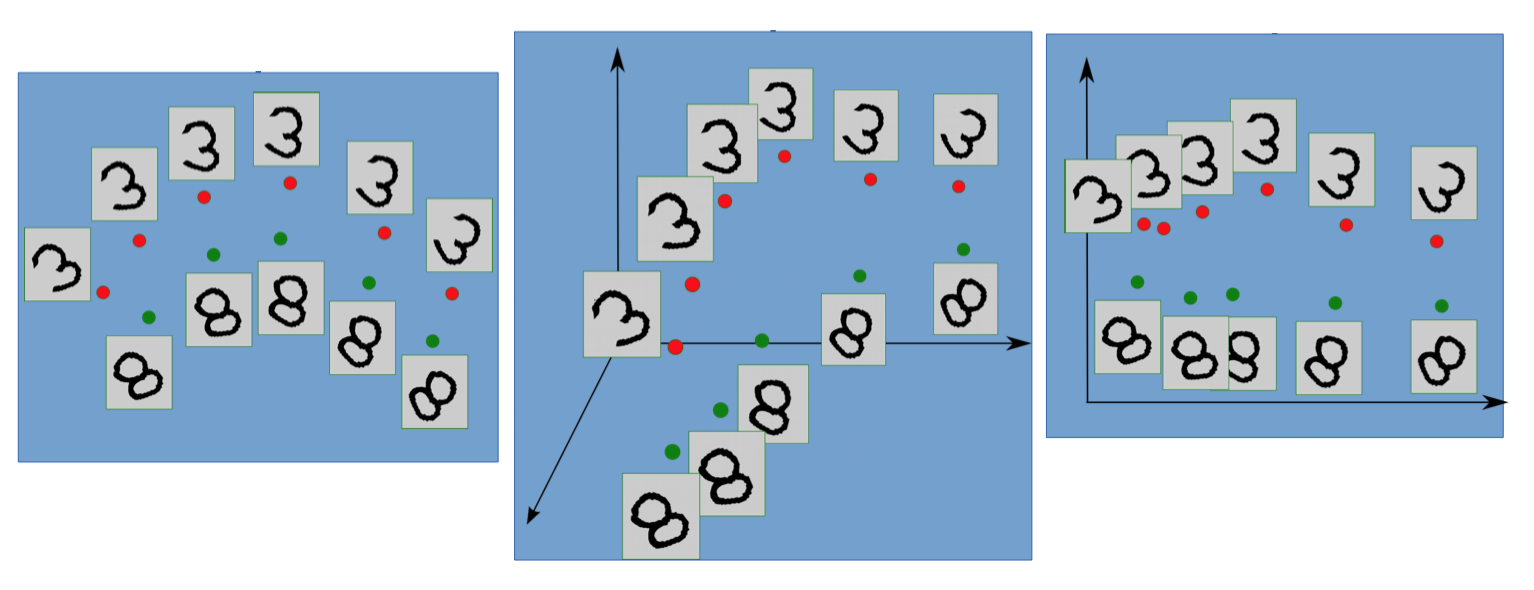
\includegraphics[width=90mm]{lectures/01-b/nonlinear_expansion.png}
\caption{Nonlinear dimensionality expansion}
\label{fig:nonlinear_expansion}
\end{figure}

\section{In the Context of the Deep Learning System Architecture}
% Authors: Hongyu (Florence) Lu, Michael Gold, Erica Dominic.
% Lecture date: 1.28.19

\Cref{sec: expand_dim} outlined the process of expanding dimensionality in a nonlinear fashion.
Here are those same steps again, this time in the context of the overall architecture for a deep learning system:
\begin{enumerate}
    \item Begin with a representation of input data
    \item Normalize the input (mean $= 0$, standard deviation $= 1$)
    \item Linearly expand the dimension (this can be done by multiplying by matrix with more rows than columns)
    \item Apply a nonlinear transformation to each component of the vector
    \item Compress the data back into a smaller dimension (linearly or with pooling)
\end{enumerate}
This process can be repeated multiple times.
